\subsection{Case02 - Pass}
\label{xdp_ether_case02}

En este caso de uso se probará que es posible admitir todos los paquetes recibidos en la interfaz donde está anclado el programa \gls{xdp}. Pero podría surgir la siguiente pregunta: ¿qué significa ``Admitir”? Se quiere comprobar si es posible dejar pasar los paquetes, sin que les afecte el datapath programado con la tecnología. El motivo es que, aunque \gls{xdp} se concibe normalmente como como un mecanismo para hacer un \textit{by-pass} al \textit{stack} de red del Kernel de Linux (es decir, una completa redefinición del mismo), en muchas ocasiones será útil trabajar en conjunto para conseguir la funcionalidad deseada. \\
\par
Para la realizar la prueba, al igual que en el case01 (\ref{xdp_ether_case01}) primero se deberá compilar el programa \gls{xdp}, acto seguido levantar el escenario donde se va a realizar la prueba, y por último, anclar el binario a una interfaz del escenario.

\begin{lstlisting}[language=C, style=C-color, caption={Programa básico XDP - Case01},label=code:case02_xdp_ether_kernprog]
    SEC("xdp_case02")
    int xdp_pass_func(struct xdp_md *ctx)
    {
    	int action = XDP_PASS;
    	goto out;
    out:
            return xdp_stats_record_action(ctx, action);
    }
    
    char _license[ ] SEC("license") = "GPL";
\end{lstlisting}
\vspace{0.5cm}

Como se puede ver en el bloque \ref{code:case02_xdp_ether_kernprog}, el programa es exactamente igual al desarrollado en el case01 (\ref{xdp_ether_case01}) cambiando únicamente el código de retorno \gls{xdp}. De esta forma se consigue modificar la funcionalidad del programa, a la deseada.\\

\vspace{0.3cm}
\textbf{Compilación}\\
\par

Para compilar el programa \gls{xdp} se ha dejado un Makefile preparado en este directorio al igual que en el case01 (\ref{xdp_ether_case01}), por lo que para compilarlo únicamente hay que seguir las indicaciones del bloque \ref{code:case02_xdp_ether_compilacion}.

\begin{lstlisting}[language= bash, style=Consola, caption={Compilación programa XDP - Case02},label=code:case02_xdp_ether_compilacion]
    # En caso de no haber entrado en el directorio asignado del caso de uso
    cd TFG/src/use_cases/xdp/case02
    
    
    # Hacemos uso del Makefile suministrado 
    sudo make
\end{lstlisting}
\vspace{0.5cm}

Ahora bien, en el anterior caso de uso no se quiso incidir demasiado en este aspecto, pero ¿Cómo se produce la compilación de los programas \gls{xdp}?  Como ya se ha podido ver, los programas \gls{xdp} están escritos en lo que llaman un lenguaje C restringido, en los cuales la secuencia de programa siempre empieza por ``xdp". Esto es así ya que, si no, el verificador del Kernel no podrá saber de que tipo de \textit{bytecode} se trata y lo rechazará.\\
\par

Este código C restringido, se compilará haciendo uso de la herramienta \textbf{clang} cómo compilador de \textit{frontend}, y de la herramienta \textbf{LLVM} cómo compilador de  \textit{backend}. De esta manera se generará un \textit{bytecode} \gls{bpf}, y posteriormente se almacenará en un objeto de tipo \gls{elf}. Estos últimos serán los que se carguen en el Kernel (\texttt{*.o}). Es curioso el hecho de entender cómo pasamos de los hipotéticos programas \gls{xdp} (C restringido) a \textit{bytecode} \gls{bpf}, ya que, cuando se indaga un poco más en \gls{xdp}, se llega a la conclusión de que \gls{xdp} se podría ver como un \textit{framework} de \gls{bpf} para trabajar a nivel de \gls{nic}.\\
\par
Hay más factores que lo diferencian de los programas \gls{bpf}, como son las estructuras de datos que manejan, además de los metadatos; pero al fin y al cabo, para anclar un programa \gls{xdp} este debe antes ser traducido a un \textit{bytecode} \gls{bpf}.\\

\vspace{0.7cm}
\textbf{Puesta en marcha del escenario}\\
\par

Para testear los programas \gls{xdp} se hará uso de las \textit{Network Namespaces} (más información en la sección \ref{namespaces}). Como ya se comentaba, para que no suponga una barrera de entrada el concepto de las \textit{Network Namespaces}, se ha dejado escrito un script para levantar el escenario, y para su posterior limpieza. Es importante señalar que el script debe ser lanzado con permisos de root. Para levantar el escenario se debe ejecutar dicho script como se indica en el bloque \ref{code:case02_xdp_ether_escenario}.\\
\par
Para limpiar la máquina del escenario recreado anteriormente, se puede correr el mismo script indicándole ahora el parámetro \texttt{-c} (\textit{Clean}). En el peor de los casos, y si se cree que la limpieza se no se ha realizado de manera satisfactoria, se puede llevar a cabo un reinicio de la máquina consiguiendo así que todos los entes no persistentes (\gls{veth}, netns..) desaparezcan del equipo.

\begin{lstlisting}[language= bash, style=Consola, caption={Puesta en marcha del escenario - Case02},label=code:case02_xdp_ether_escenario]
    # Para levantar el escenario (Importante hacerlo con permisos de super usuario)
    sudo ./runenv.sh -i
    
    
    # Una vez finalizado la comprobación del caso de uso, limpiaremos nuestra maquina:
    sudo ./runenv.sh -c
\end{lstlisting}
\vspace{0.5cm}

El escenario que se va a manejar en este caso de uso es el siguiente (Ver figura \ref{fig:case02_xdp_ether_scenario}), compuesto únicamente de una \textit{Network Namespace} (\texttt{uno}) y un par de \gls{veth}s (\texttt{veth0} -- \texttt{uno}) para comunicar la \textit{Network Namespace} creada con la \textit{Network Namespace} por defecto.

\newpage

% figura escenario
\begin{figure}[ht]
    \centering
    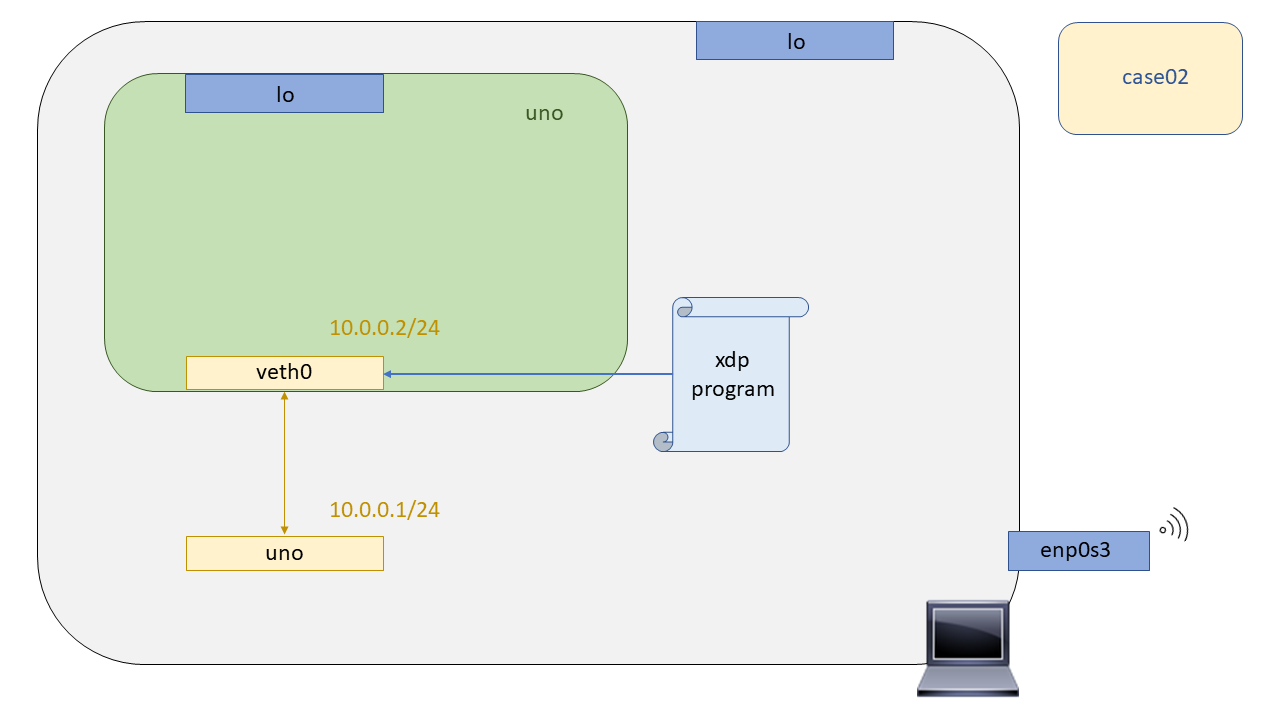
\includegraphics[width=16cm]{archivos/img/dev/xdp/case02/scenario.png}
    \caption{Escenario cableado del Case02 - XDP}
    \label{fig:case02_xdp_ether_scenario}
\end{figure}

\vspace{0.5cm}
\textbf{Carga del programa \gls{xdp}}\\
\par
Una vez que se tiene el escenario y el programa \gls{xdp} compilado, se procederá a cargarlo en el Kernel. Para más información sobre el programa  xdp\_loader, qué aporta la librería libbpf, o por que no se hace uso de la herramienta iproute2 para cargar los programas \gls{xdp} en el Kernel, se recomienda regresar al case01 (\ref{xdp_ether_case01})  donde se intenta abordar todas estas cuestiones.\\
\par

Como se comentaba, es hora de cargar el programa en el Kernel, esta vez por variar se va a cargar el programa \gls{xdp} en el extremo de la \gls{veth} que se encuentra en el interior de la \textit{Network Namespace}. Se podría haber hecho de la misma manera que en el caso de uso anterior y cargar el programa \gls{xdp} en la \gls{veth} que se ve desde la \textit{Network Namespace} por defecto, pero de esta manera se explorará como ejecutar comandos ``dentro" de una \textit{Network Namespace}. Para ejecutar comandos ``dentro" de una \textit{Network Namespace} se hará uso de la herramienta iproute2 (\ref{iproute2}), más concretamente su módulo llamado \textbf{netns}. A la herramienta se le debe indicar el parámetro \texttt{exec} y el nombre de la \textit{Network Namespace} dónde se quiera ejecutar el comando, y por último, se le indicará el comando que correrá ``dentro" de la \textit{Network Namespace}.

\begin{lstlisting}[language= bash, style=Consola, caption={Carga del programa XDP - Case02},label=code:case02_xdp_ether_load]
    # Cargaremos el programa sobre la interfaz "veth0" 
    sudo ip netns exec uno ./xdp_loader -d veth0 -F --progsec xdp_case02
\end{lstlisting}
\vspace{0.2cm}

Por lo que, entendiendo como funciona el módulo netns, y los parámetros suministrados al programa xdp\_loader, explicados en el caso de uso case01 (\ref{xdp_ether_case01}), se podrá intuir que el resultado de la sentencia anterior es la de cargar el programa \gls{xdp} en la interfaz llamada \texttt{veth0} contenida en la \textit{Network Namespace} \texttt{uno}.


\vspace{1.2cm}
\textbf{Comprobación del funcionamiento}\\
\par


La comprobación del funcionamiento del programa \gls{xdp} anclado a la interfaz \texttt{veth0} se llevará a cabo testeando la conectividad entre el par de \gls{veth}s. Puede que sea una prueba un poco simple, pero es suficiente, ya que únicamente se quiere verificar que el programa anclado en la interfaz está delegando los paquetes que le llegan, al \textit{stack} de red.\\
\par

En este punto se quiere comentar un aspecto de \gls{xdp}, y es que, desde que se empezó a trabajar con \gls{xdp}, se veía al \textit{stack} de red de Linux como a un enemigo a batir, o ``by-passear"; ya que con \gls{xdp} se quiere conseguir definir de manera exclusiva el datapath que se desea implementar con un equipo que porte el Kernel de Linux.  De esta manera, se consigue técnicamente un rendimiento superior ya que se quita de encima toda la redundancia y capas que no son necesarias para el procesamiento del hipotético datapath.\\
\par
Ahora bien, en el transcurso del aprendizaje con esta tecnología se ha visto que en ocasiones trabajar de manera cooperativa con el \textit{stack} de red puede reportar muchas facilidades y muchas otras funcionalidades ya implementadas en éste. No es cuestión de reinventar la rueda, más que nada porque el rendimiento que se puede llegar a ganar por hacer todo el procesamiento de manera exclusiva en la propia \gls{nic}, en opinión del autor, no compensa con la robustez y fiabilidad que tendrá dicha funcionalidad en el \textit{stack} de red de Linux.\\
\par
Como se puede apreciar en la figura \ref{fig:case02_xdp_ether_func}, prestando atención al ping \fcolorbox{black}{green}{\rule{0pt}{2.5pt}\rule{2.5pt}{0pt}}  (Fig. \ref{fig:case02_xdp_ether_func_ping}), hay perfecta conectividad. Eso significa que el programa \gls{xdp} está delegando correctamente los paquetes al \textit{stack} de red, se puede verificar dicho funcionamiento atendiendo a las estadísticas sobre los códigos de retorno de la figura \ref{fig:case02_xdp_ether_func_stats}, dónde el código de retorno \texttt{XDP\_PASS} va en aumento. Dichas estadísticas han sido recolectadas haciendo uso del binario xdp\_stats. En el siguiente caso de uso se explicará brevemente el funcionamiento de la recolección de estadísticas de los programas \gls{xdp}. 
\newpage

\begin{figure}[h!]
    \centering
    \begin{subfigure}[b]{\textwidth}
    	\centering
        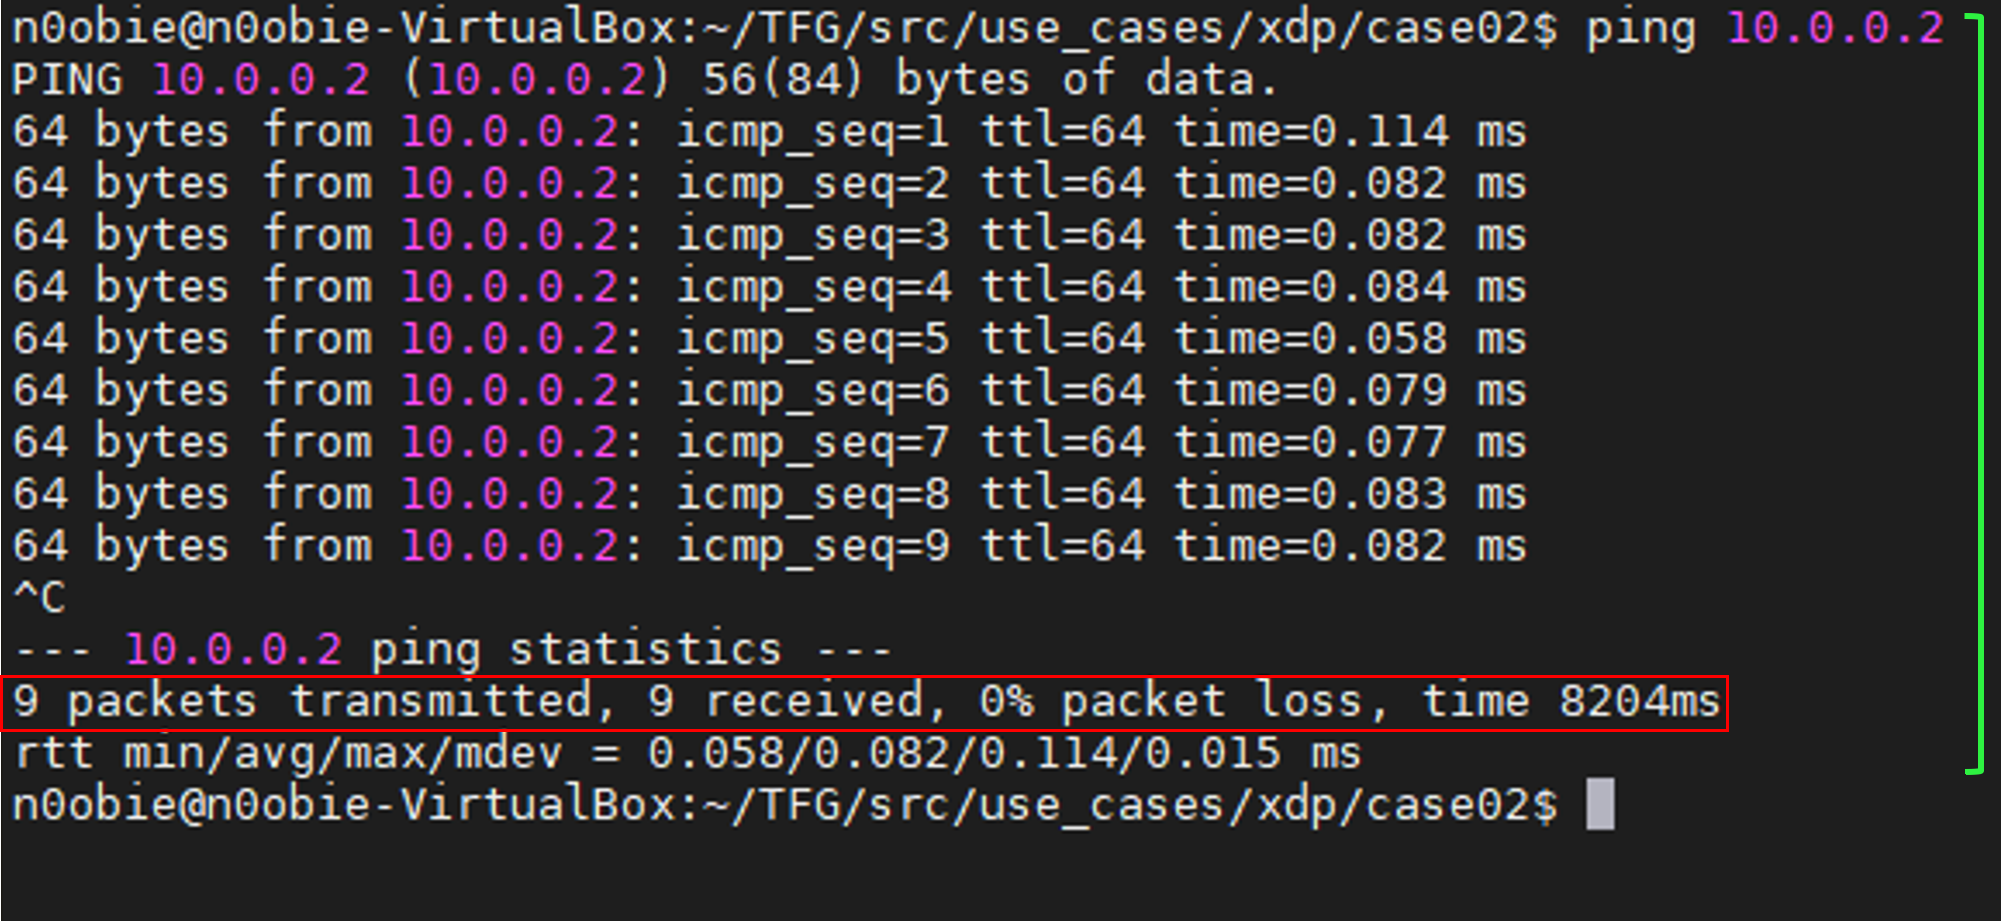
\includegraphics[width=11cm]{archivos/img/dev/xdp/case02/demo_case02_3_edited.png}
        \caption{Ejecución de ping hacia la interfaz con el programa XDP}
        \label{fig:case02_xdp_ether_func_ping}
    \end{subfigure}
    \par\bigskip
    \begin{subfigure}[b]{\textwidth}
    	\centering
    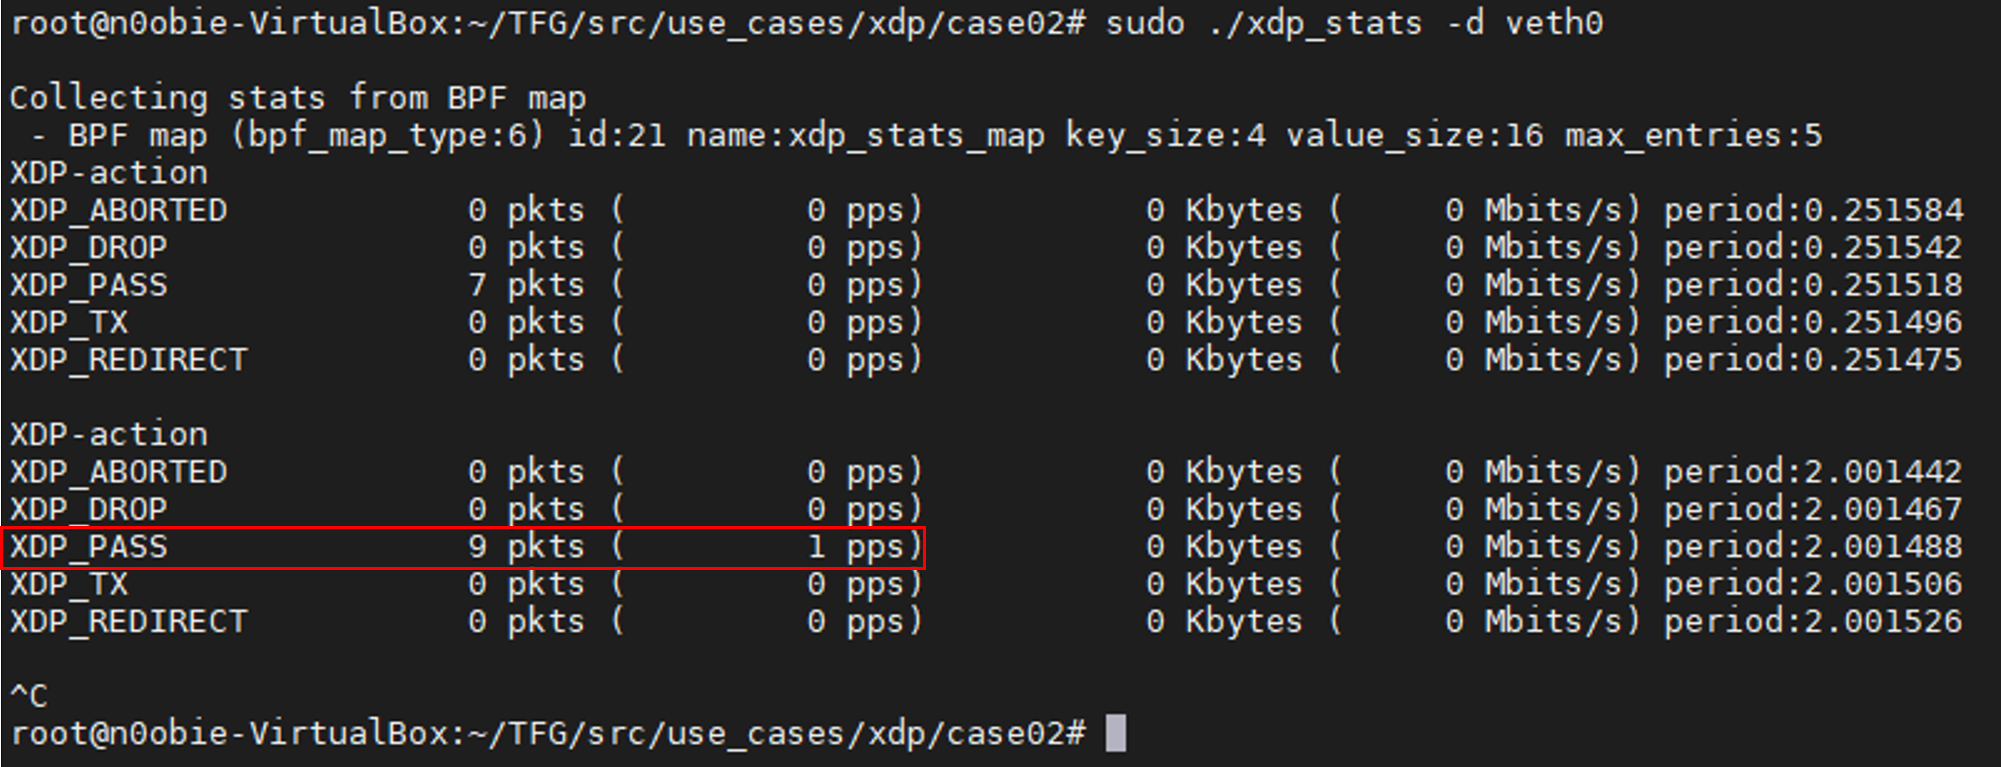
\includegraphics[width=14cm]{archivos/img/dev/xdp/case02/demo_case02_4_edited.png}
        \caption{Estadísticas de los códigos de retorno XDP}
        \label{fig:case02_xdp_ether_func_stats}
    \end{subfigure}
    \caption{Comprobación de funcionamiento del Case02 - XDP}
    \label{fig:case02_xdp_ether_func}
\end{figure}

